\documentclass{article}
\usepackage[utf8]{inputenc}
\usepackage{graphicx} %package to manage images
\graphicspath{ {./images/} }
\usepackage{wrapfig}
\title{Neumorphism Calculator with HTML and CSS}
\author{Andreea Draghici }
\date{April 2021}
\begin{document}
\maketitle
\section{Task:}
\paragraph{Make a neumorphism calculator using html and css.}
\paragraph{This neumorphism calculator performs a simple arithmetic operations, such as addition, difference, multiplication, division.\\
We also find an option to check if a number is smaller than another number.}
\begin{figure}[h]
    \centering
    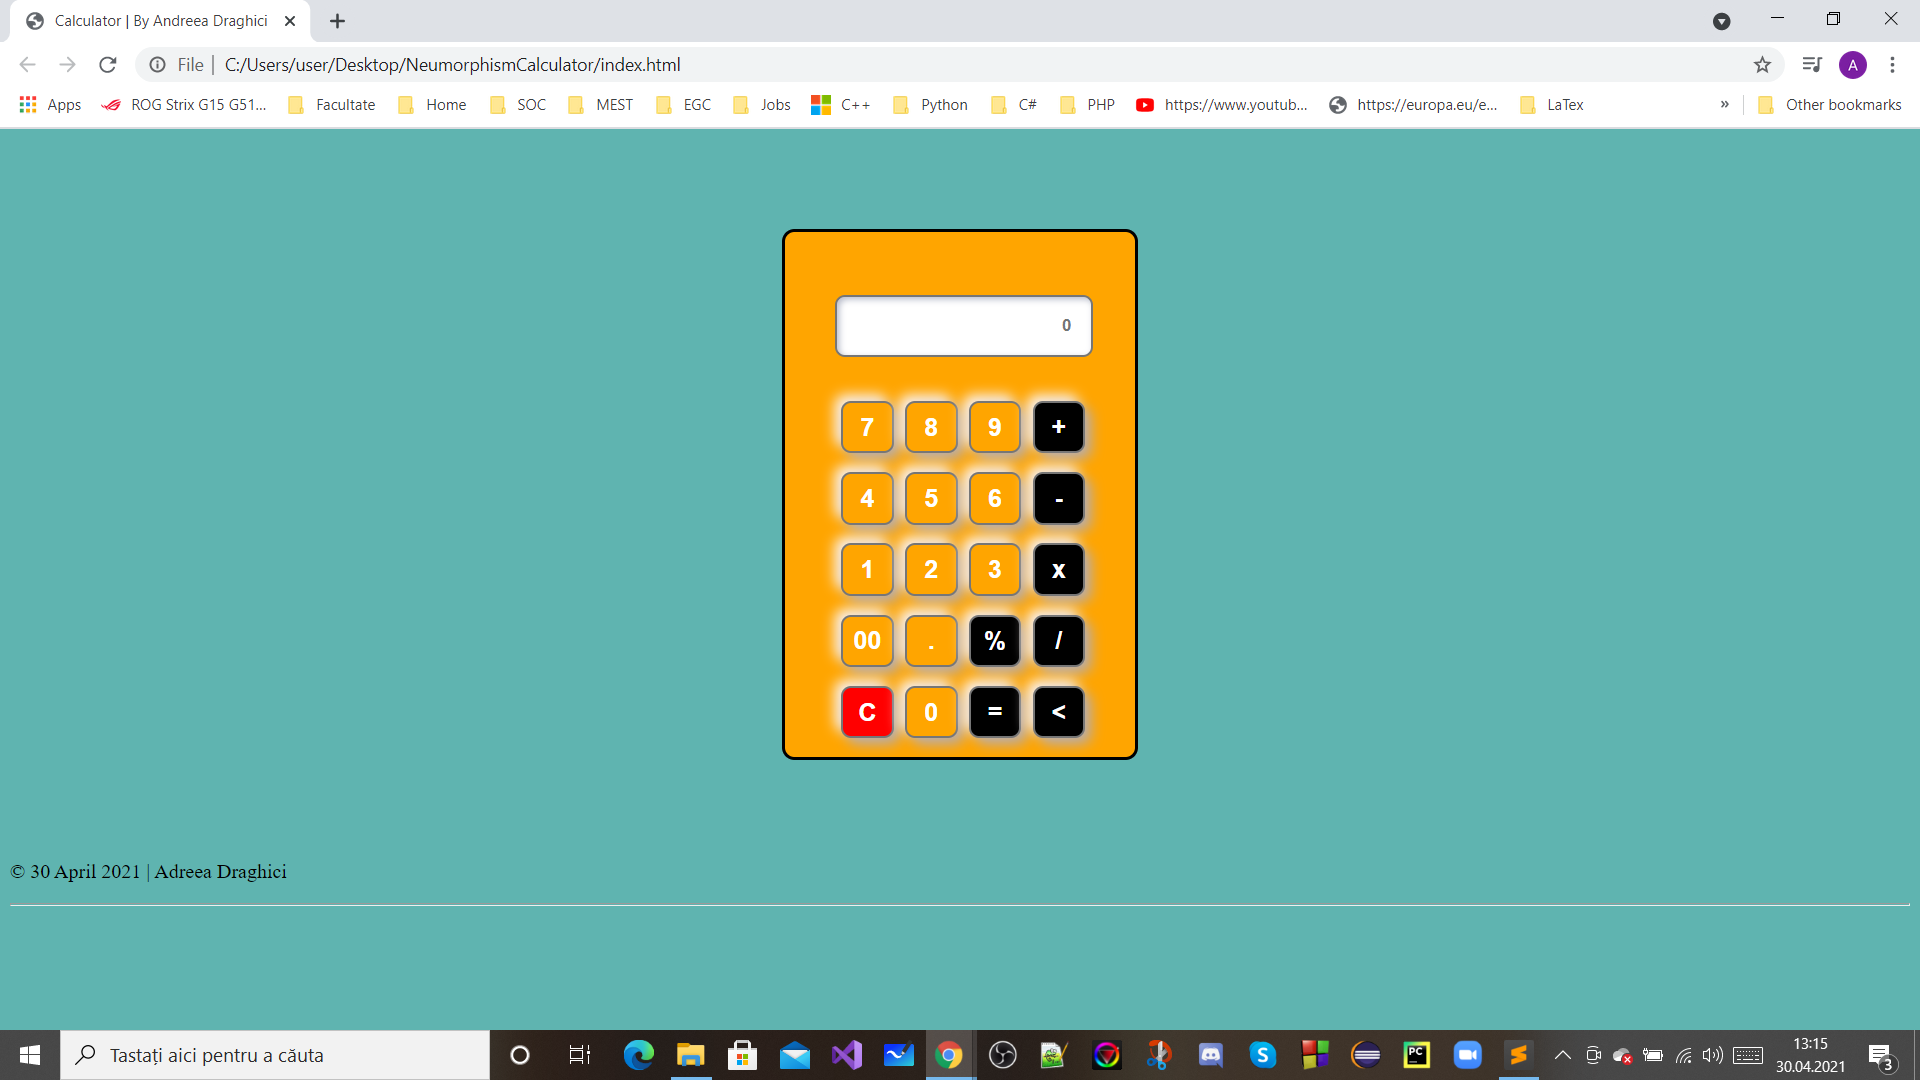
\includegraphics[width=15cm]{first.png}
    \caption{The appearance of the neumorphism calculator }
    \label{first.png}
\end{figure}
\newpage
\begin{figure}[h]
    \centering
    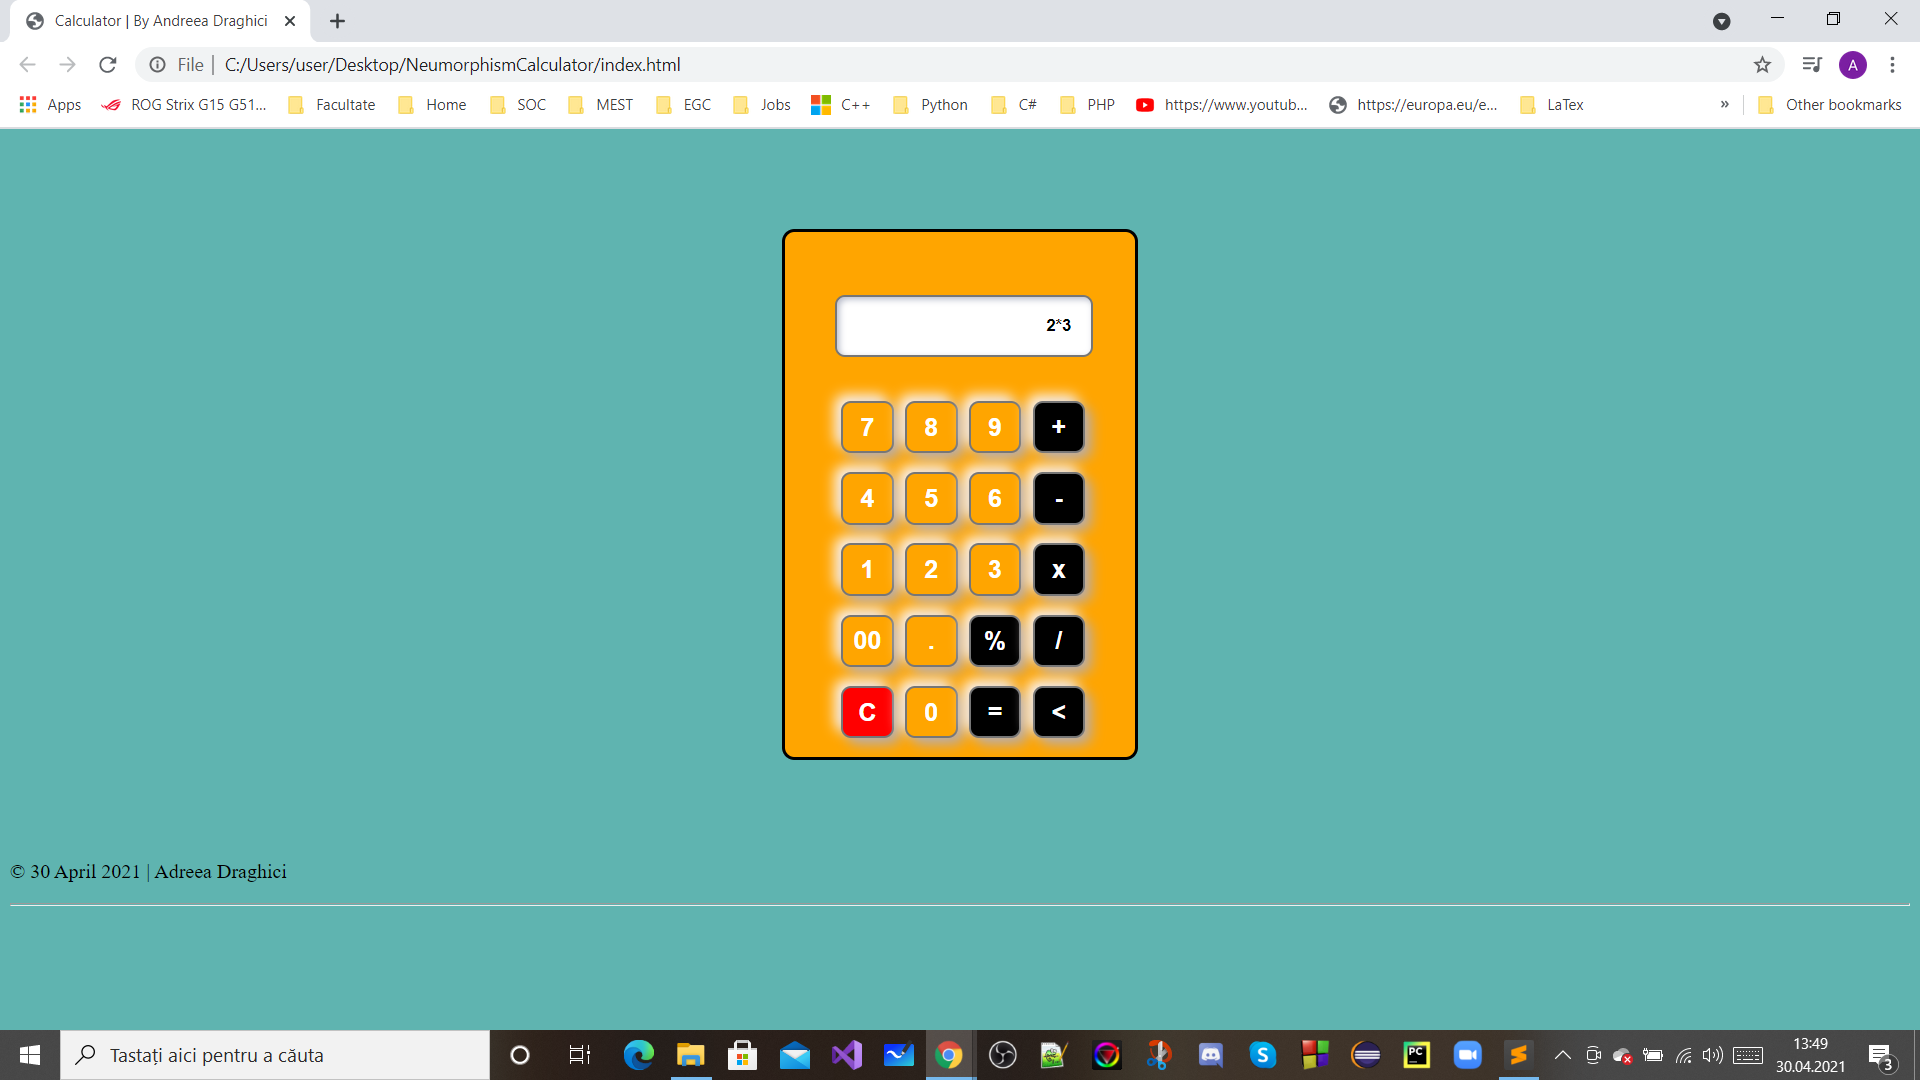
\includegraphics[width=15cm]{inmultire.png}
    \caption{Multiplication operation}
    \label{inmultire.png}
\end{figure}
\vspace{1.5cm}
\begin{figure}[h]
    \centering
    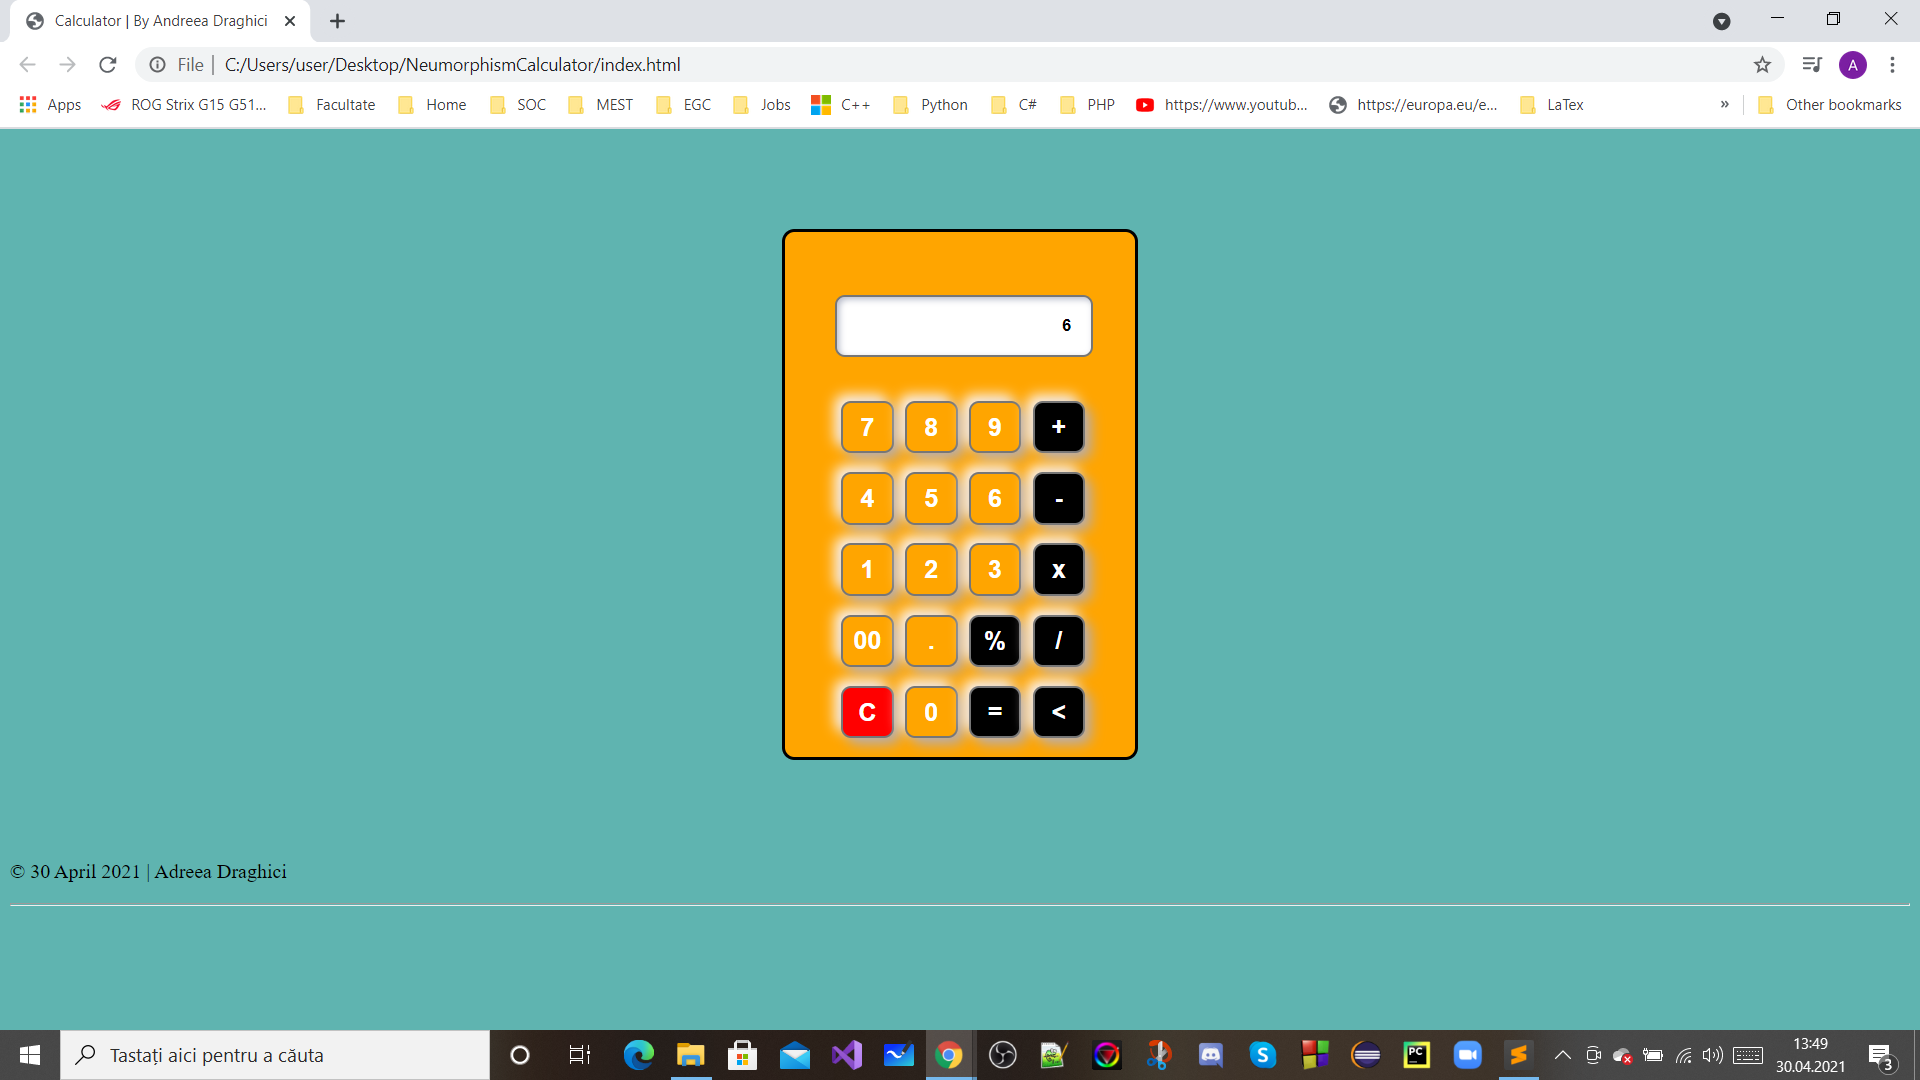
\includegraphics[width=15cm]{rezultat.png}
    \caption{Result of multiplication operation}
    \label{inmultire.png}
\end{figure}
\newpage
\paragraph{This is a mini project for personal development accumulating basic notions in css and html.\\\\
I used the introductory notions from the w3schools site, both for css and html.\\\\}
\begin{thebibliography}{}
\bibitem{w3schools site} 
\\\texttt{https://www.w3schools.com/\css/\\}
\end{thebibliography}
\end{document}